\documentclass[12pt]{article}
\usepackage[utf8]{inputenc}
\usepackage[left=2cm,right=2cm,top=2cm,bottom=2cm]{geometry}
\usepackage{graphicx}
\usepackage[small]{caption}
\usepackage{subcaption}
\usepackage[spanish]{babel}
\usepackage{url}
\setlength{\parskip}{\baselineskip}
\graphicspath{ {images/} }


\usepackage{hyperref}
\hypersetup{
	colorlinks=true,
	linkcolor=blue,     
	urlcolor=blue,
	citecolor=blue,
}

\spanishdecimal{.}

\begin{document}


	\thispagestyle{empty}

	\begin{center}
		{\Large \bf Distribución de Poisson}\\
		Gabriela S\'anchez Y.\\
		5064
	\end{center}
 
	En el presente trabajo se realiza un estudio de las formas en que se puede aproximar la distribución de Poisson usando otro tipo de distribuciones. La experimentación para las aproximaciones se realiza con la ayuda del lenguaje de programación \textsc{R} versión 4.0.2 \cite{r}. El código puede encontrarse en el archivo \texttt{t4.R} \cite{mpa_gaby}.

	%\section{Distribución de Poisson}
	

	\section{Distribución de Poisson a partir de la distribución binomial}
	
	El proceso que se sigue para llegar a una aproximación a la distribución de Poisson a partir de la distribución binomial es el siguiente: se suman valores provenientes de una distribución binomial con parámetros  $n=10000$ y $p=0.001$, y se cuentan los necesarios para llegar a una {\em meta}. Los resultados son graficados y se comparan con valores obtenidos con la función  \texttt{rpois}, con parámetro $\lambda = n\cdot p$.
	
	El parámetro de la {\em meta}, así como el número de veces que se repite el experimento se variaron durante el análisis. La figura \ref{poisson_binom} muestra dos de los resultados obtenidos con un número fijo de repeticiones $r=1000$. Las formas se observan parecidas, en especial la mostrada en la figura \ref{poisson_binom-m70}. Al observar detalladamente los ejes, se advierte que la aproximación parece estar ``movida'' hacia la izquierda. Es decir, las formas no coinciden en el eje horizontal. 
	
	Analíticamente, en clase se estudió que existe una relación entre la distribución de Poisson y la distribución binomial. Si se toman valores de $n$ grandes y valores de $p$ pequeños en la distribución binomial y se define $\lambda = n\cdot p$, se cumple que la distribución binomial aproxima a la distribución de Poisson al hacer $n \rightarrow \infty$.
	
	\begin{figure}
		\begin{subfigure}{\textwidth}
			\centering
			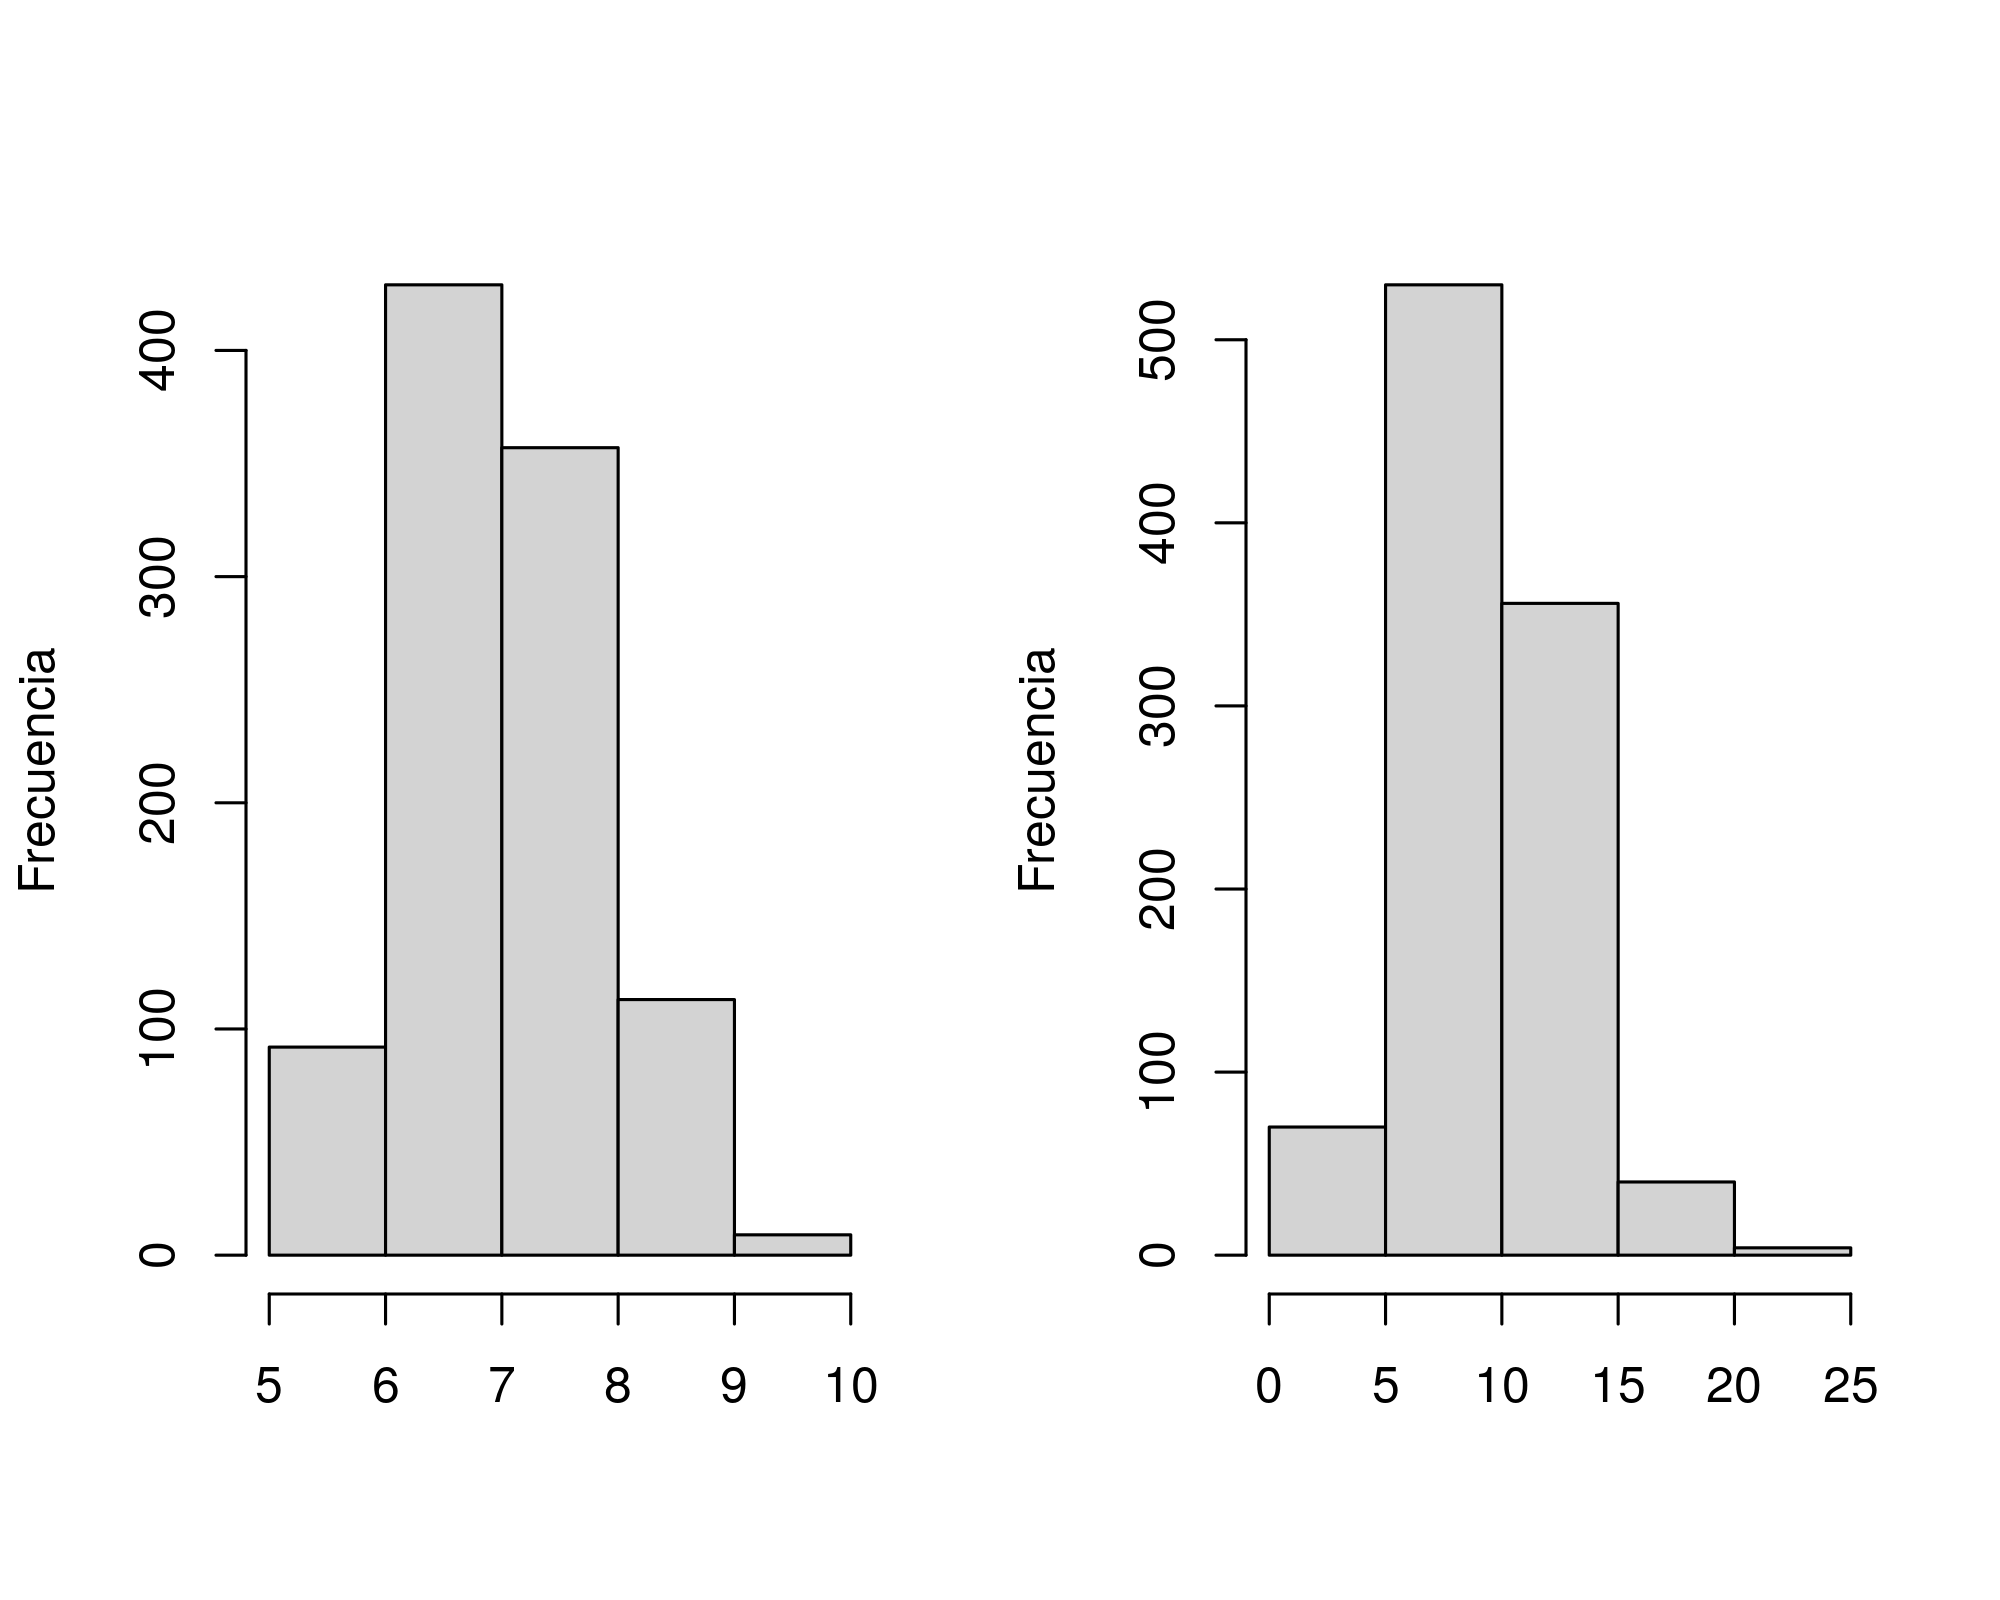
\includegraphics[scale=0.7]{poisson_binom-p001-n1000-m70-r1000.png}
			\caption{Aproximación con {\em meta} = 70.}
			\label{poisson_binom-m70}
		\end{subfigure}
	
		\begin{subfigure}{\textwidth}
			\centering
			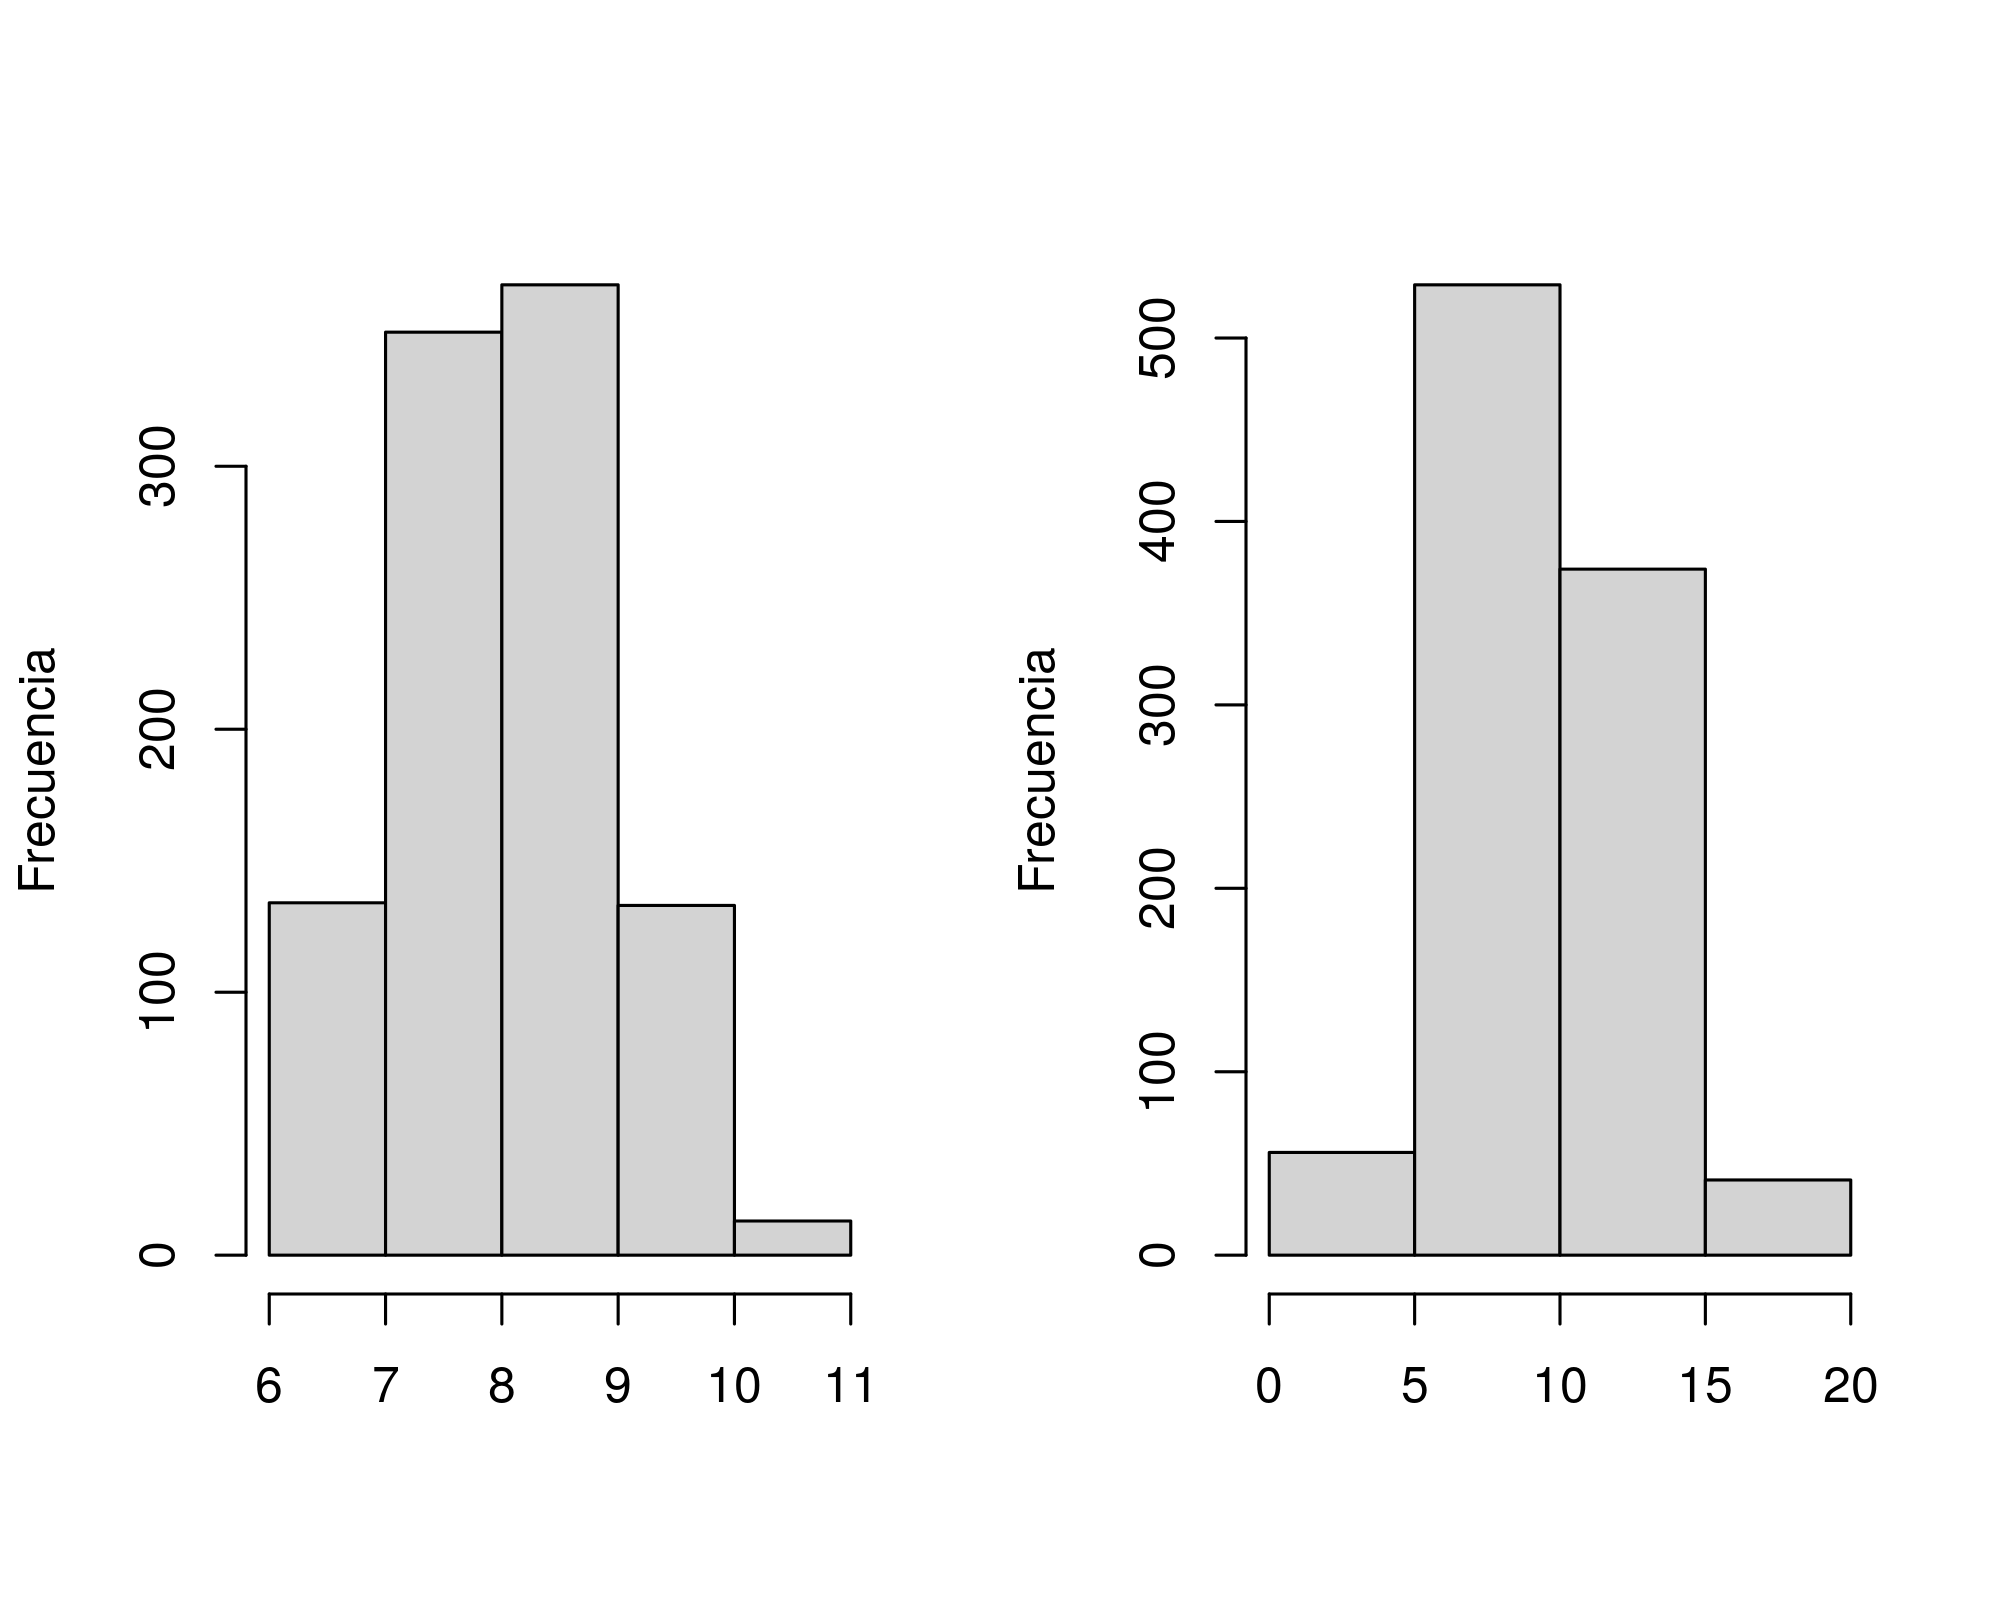
\includegraphics[scale=0.7]{poisson_binom-p001-n1000-m80-r1000.png}
			\caption{Aproximación con {\em meta} = 80.}
			\label{poisson_binom-m80}
		\end{subfigure}
		\caption{A la izquierda la aproximación a la distribución de Poisson, a la derecha la distribución de valores con la función \texttt{rpois(r, n*p)}.}
		\label{poisson_binom}
	\end{figure}
	
	\section{Distribución de Poisson a partir de una distribución normal}
	
	La idea seguida en la sección anterior se aplica también en este análisis. Es decir, se suman valores provenientes de una distribución normal con parámetros  $\mu=\lambda$ y $\sigma^2=\lambda$, y se cuentan los necesarios para llegar a una {\em meta}. La elección de estos parámetros fue combinación entre una larga experimentación y lectura sobre ambas distribuciones.
	
	La figura \ref{poisson_normal} muestra los resultados obtenidos; a la izquierda se muestra la aproximación con la distribución normal y a la derecha la distribución de valores obtenida con la función \texttt{rpois(r, l)}. En este caso $\lambda = 100$, $meta=8000$ y se repite el experimento $r=1000$ veces.
	
	\begin{figure}
		\centering
		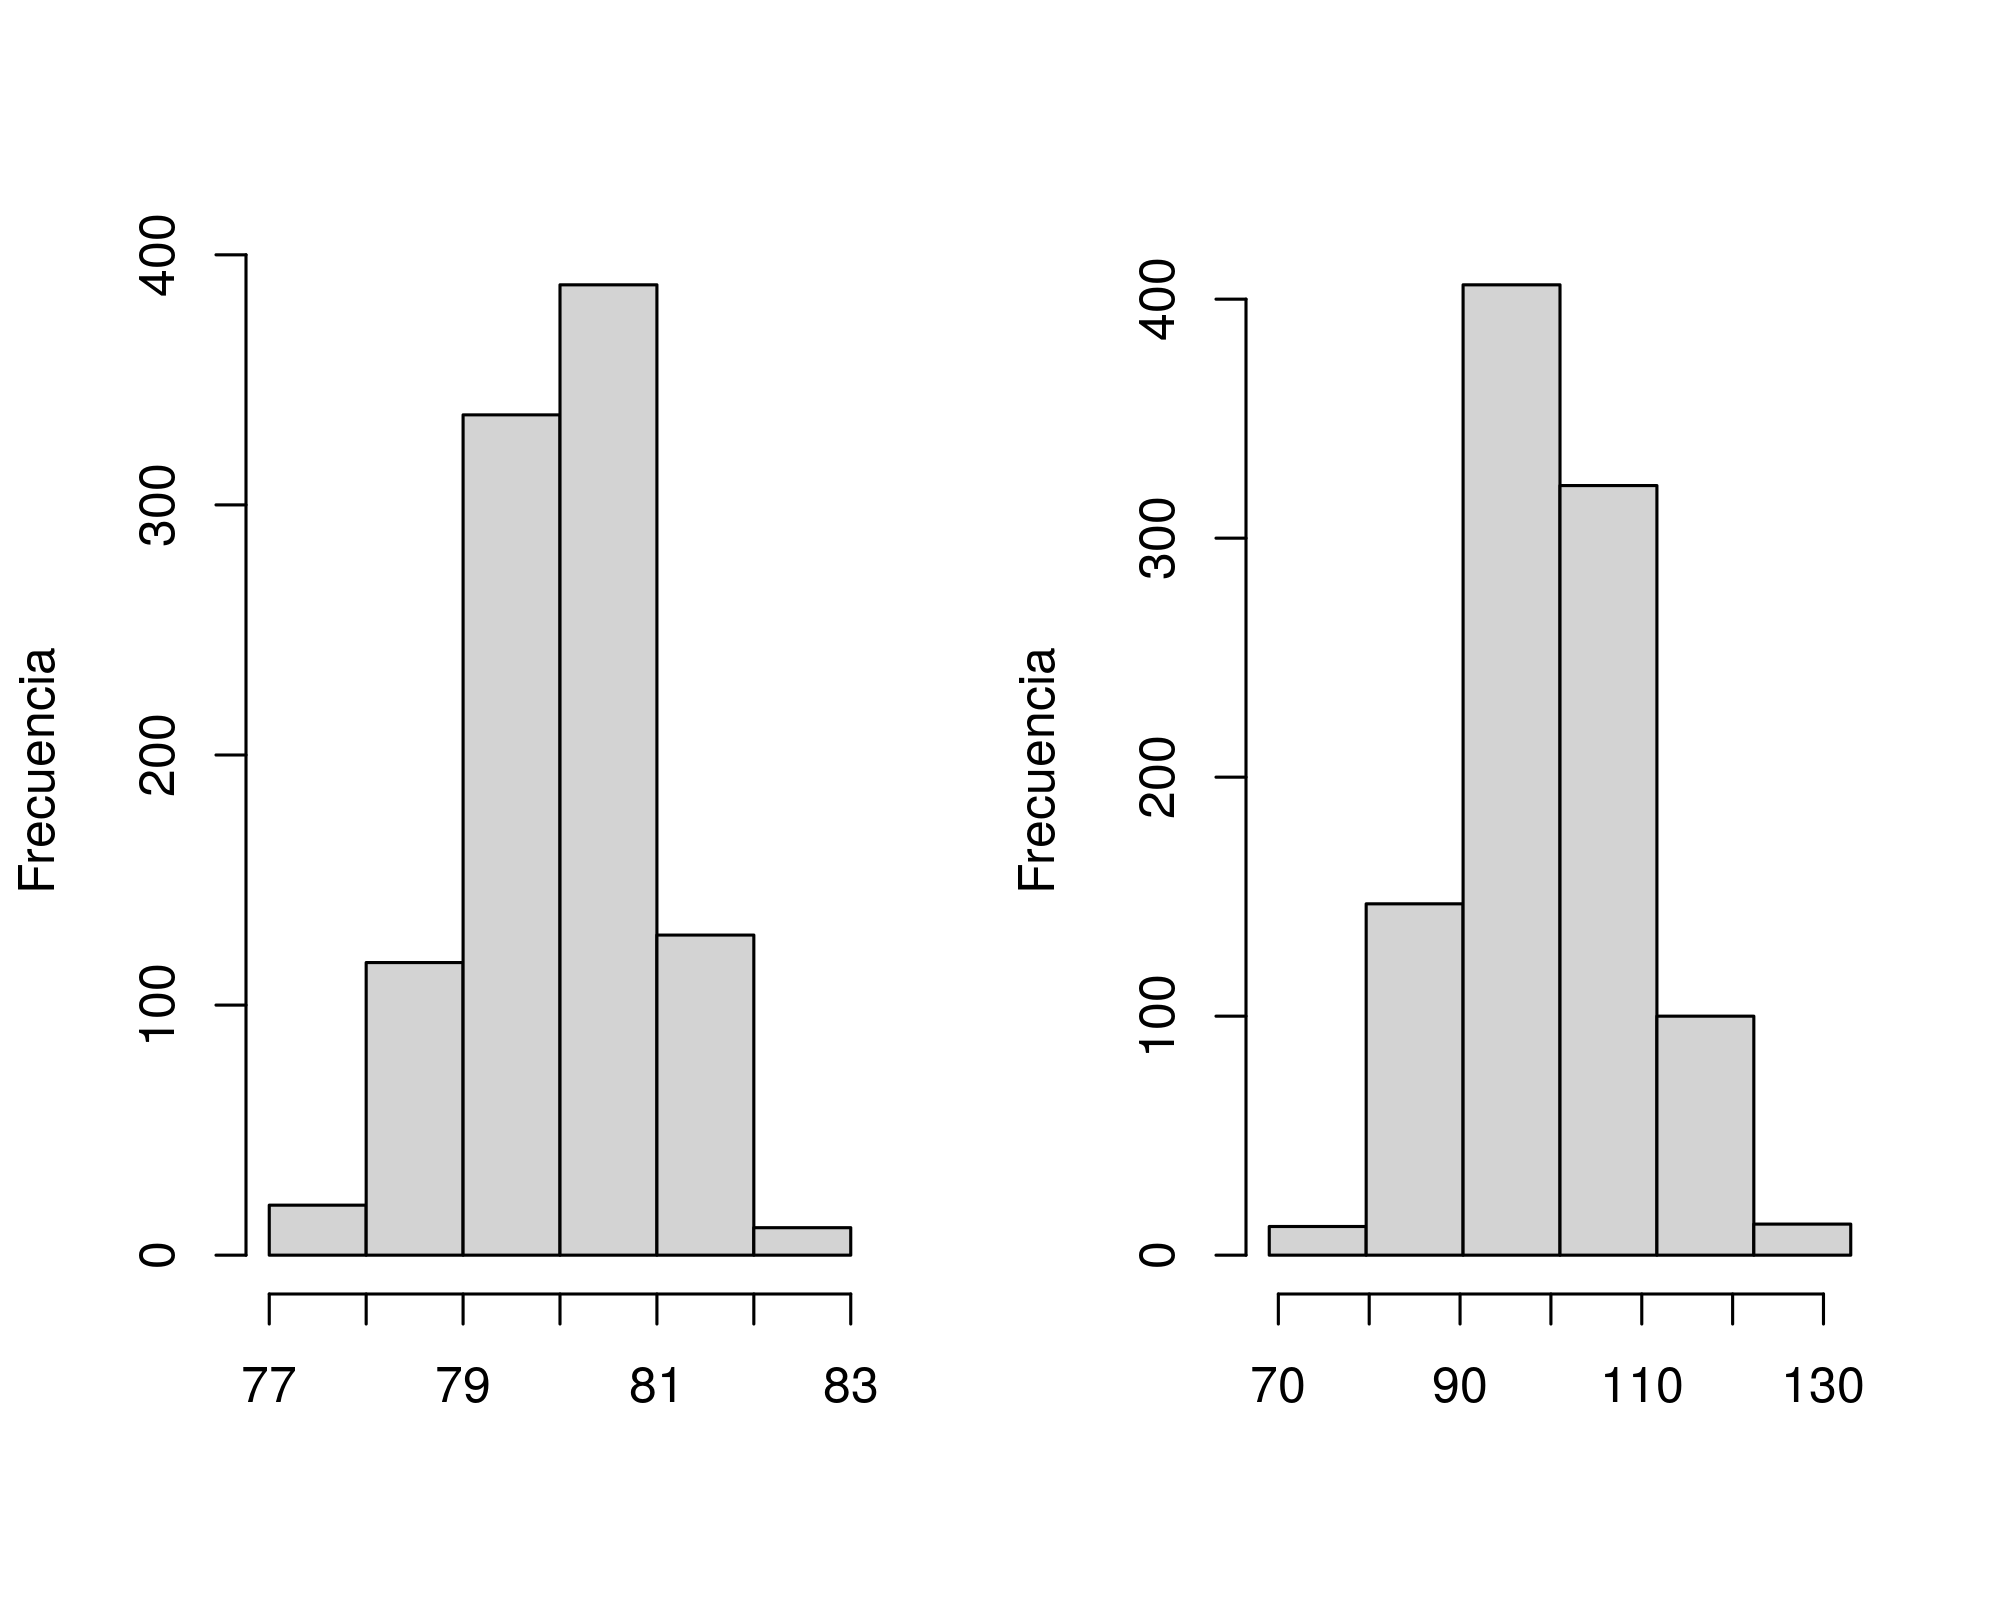
\includegraphics[scale=0.7]{poisson_normal-m8000-l100-r1000.png}
		\caption{Aproximación a la distribución de Poisson a partir de la distribución normal. A la izquierda se encuentra la aproximación y a la derecha la distribución usando \texttt{rpois(r, lambda)}.}
		\label{poisson_normal}
	\end{figure}
	
	Al analizar las formas de la figura, se puede percibir que ambas distribuciones tienen una forma similar. Sin embargo, en este caso la aproximación también esta ``movida'' hacia la izquierda. Esto claramente es resultado de la elección de parámetros.
	
	Aunque no se tiene una demostración analítica, en la figura \ref{poisson_norm_r} se muestra la distribución de $r=10000$ valores obtenidos de una distribución de Poisson de parámetro $\lambda$ y una distribución normal con $\mu = \lambda$ y $\sigma^2 = \lambda$. Nótese que a medida que el parámetro $\lambda$ aumenta, las distribuciones se asemejan más. Con esto, al menos se puede concluir que la relación entre ambas distribuciones es correcta con la elección de parámetros indicados.
	
	\begin{figure}
		\begin{subfigure}{\textwidth}
			\centering
			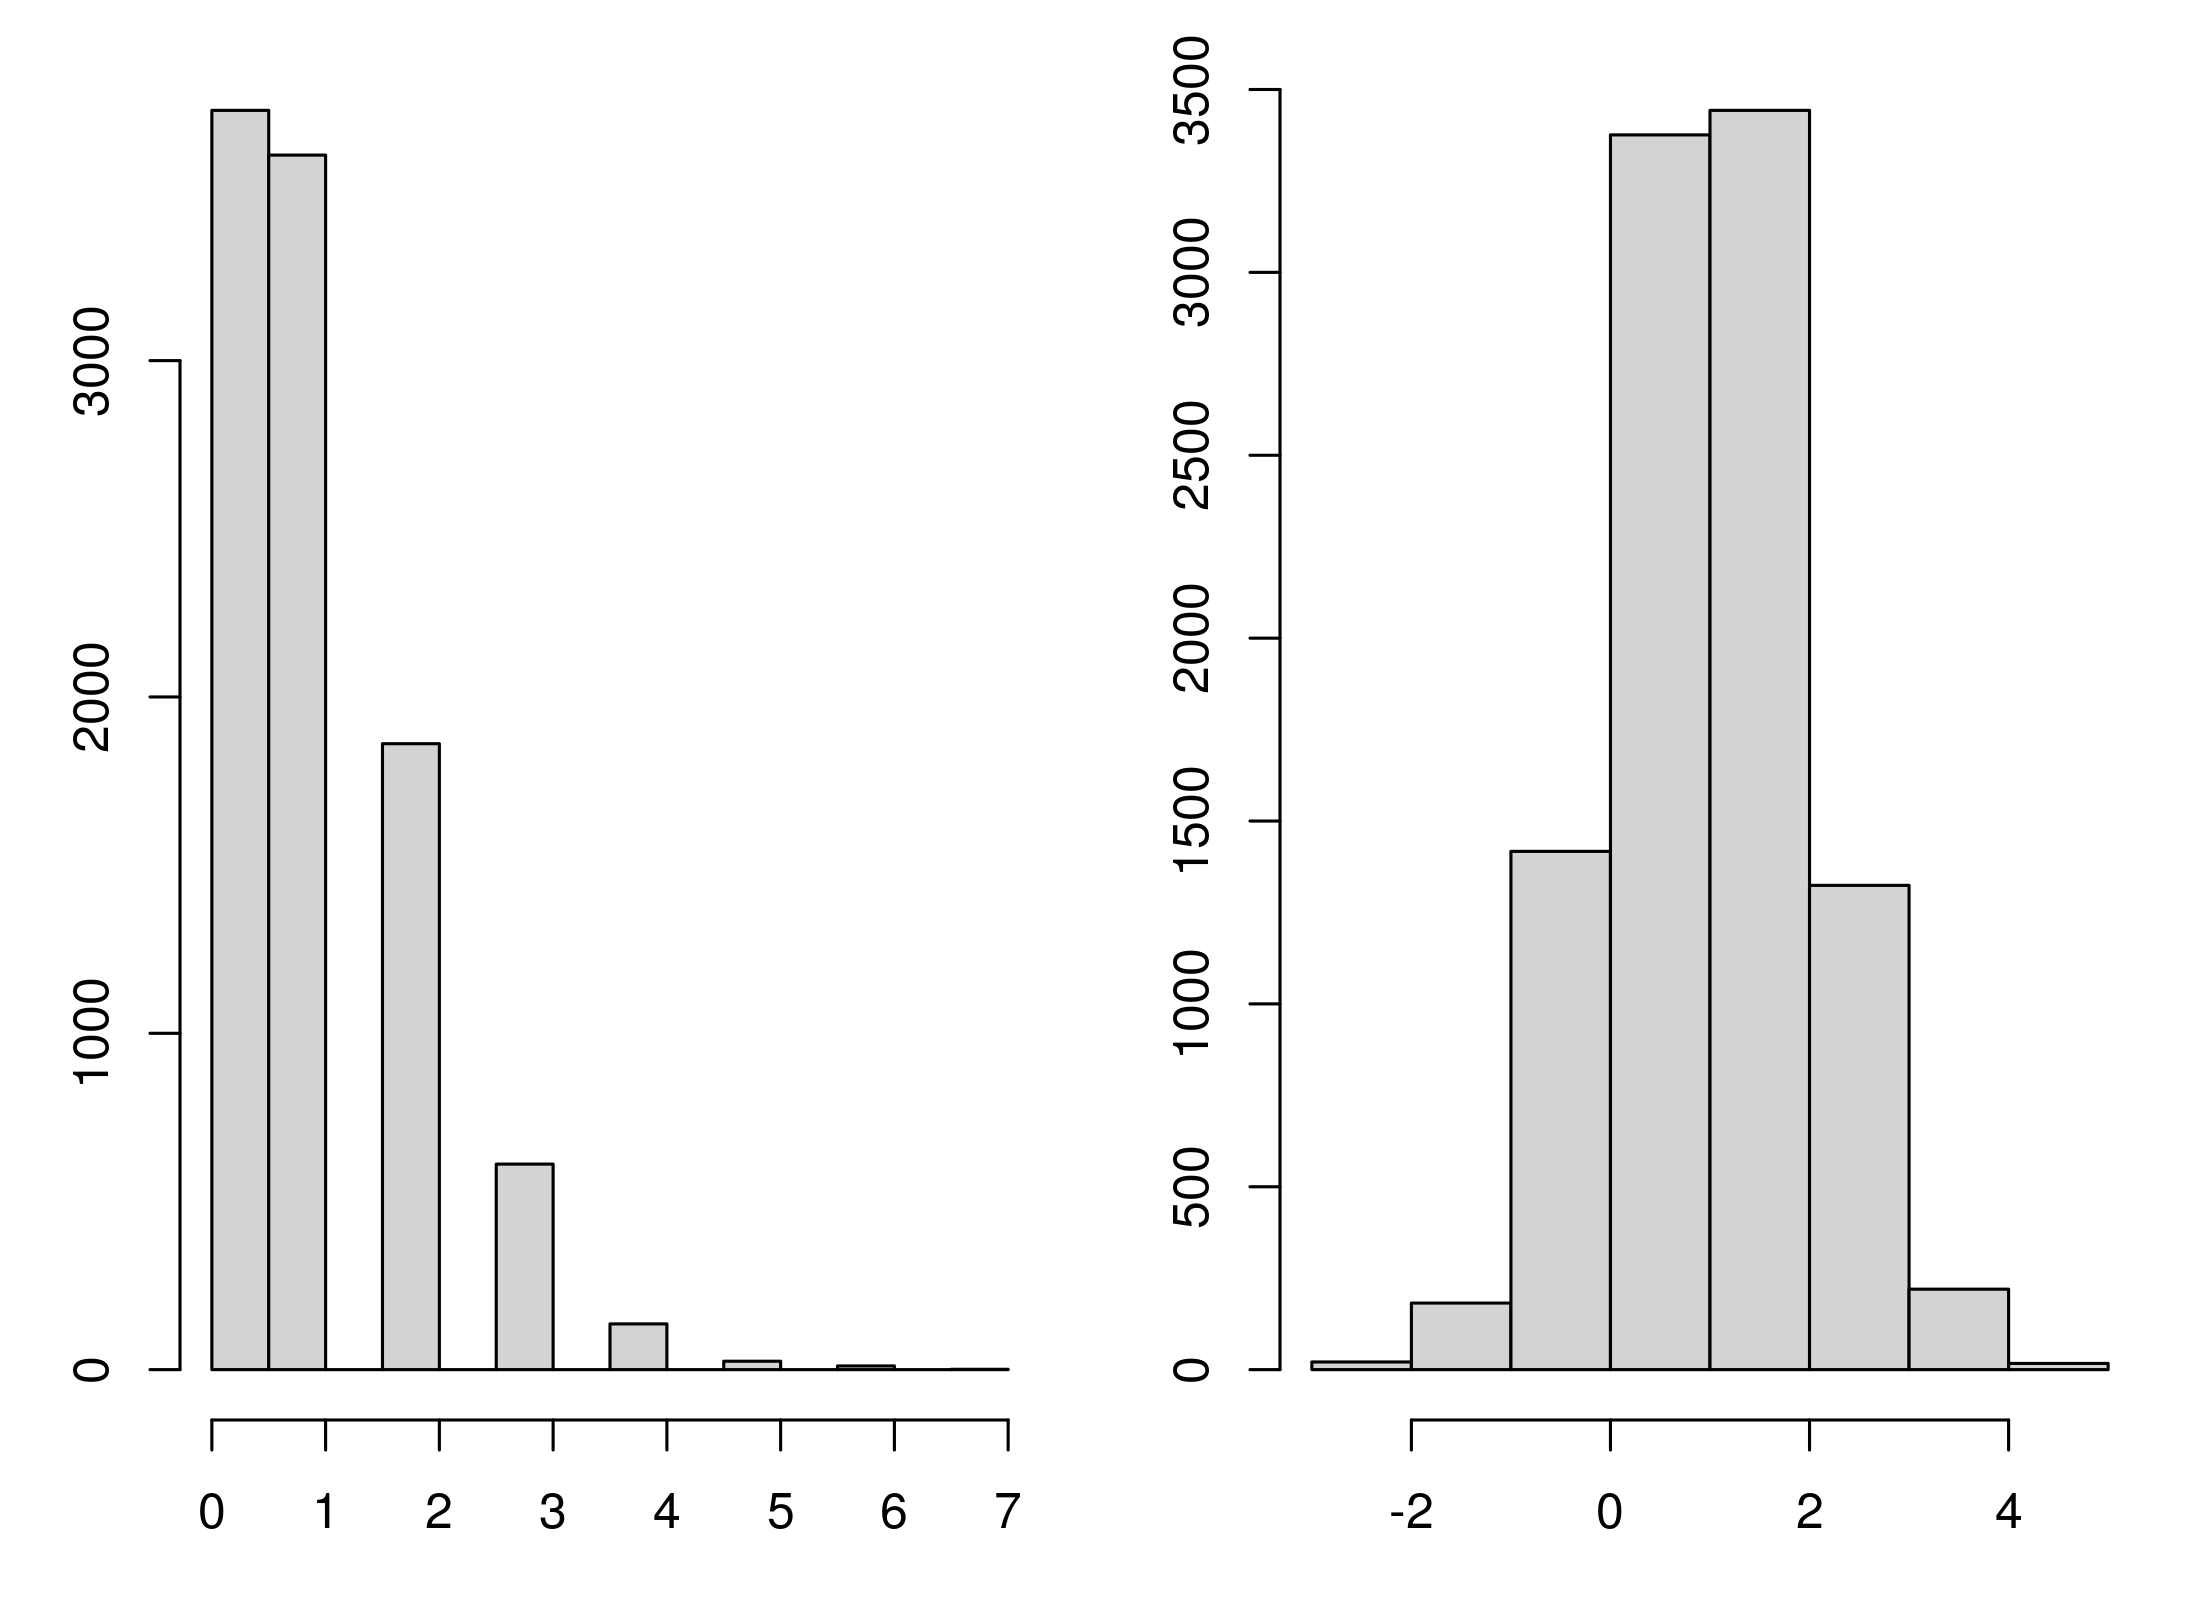
\includegraphics[width=0.5\linewidth]{poisson_normal_vl1.png}
			\caption{$\lambda = 1$.}
			\label{poisson_norm1}
		\end{subfigure}
		\begin{subfigure}{\textwidth}
			\centering
			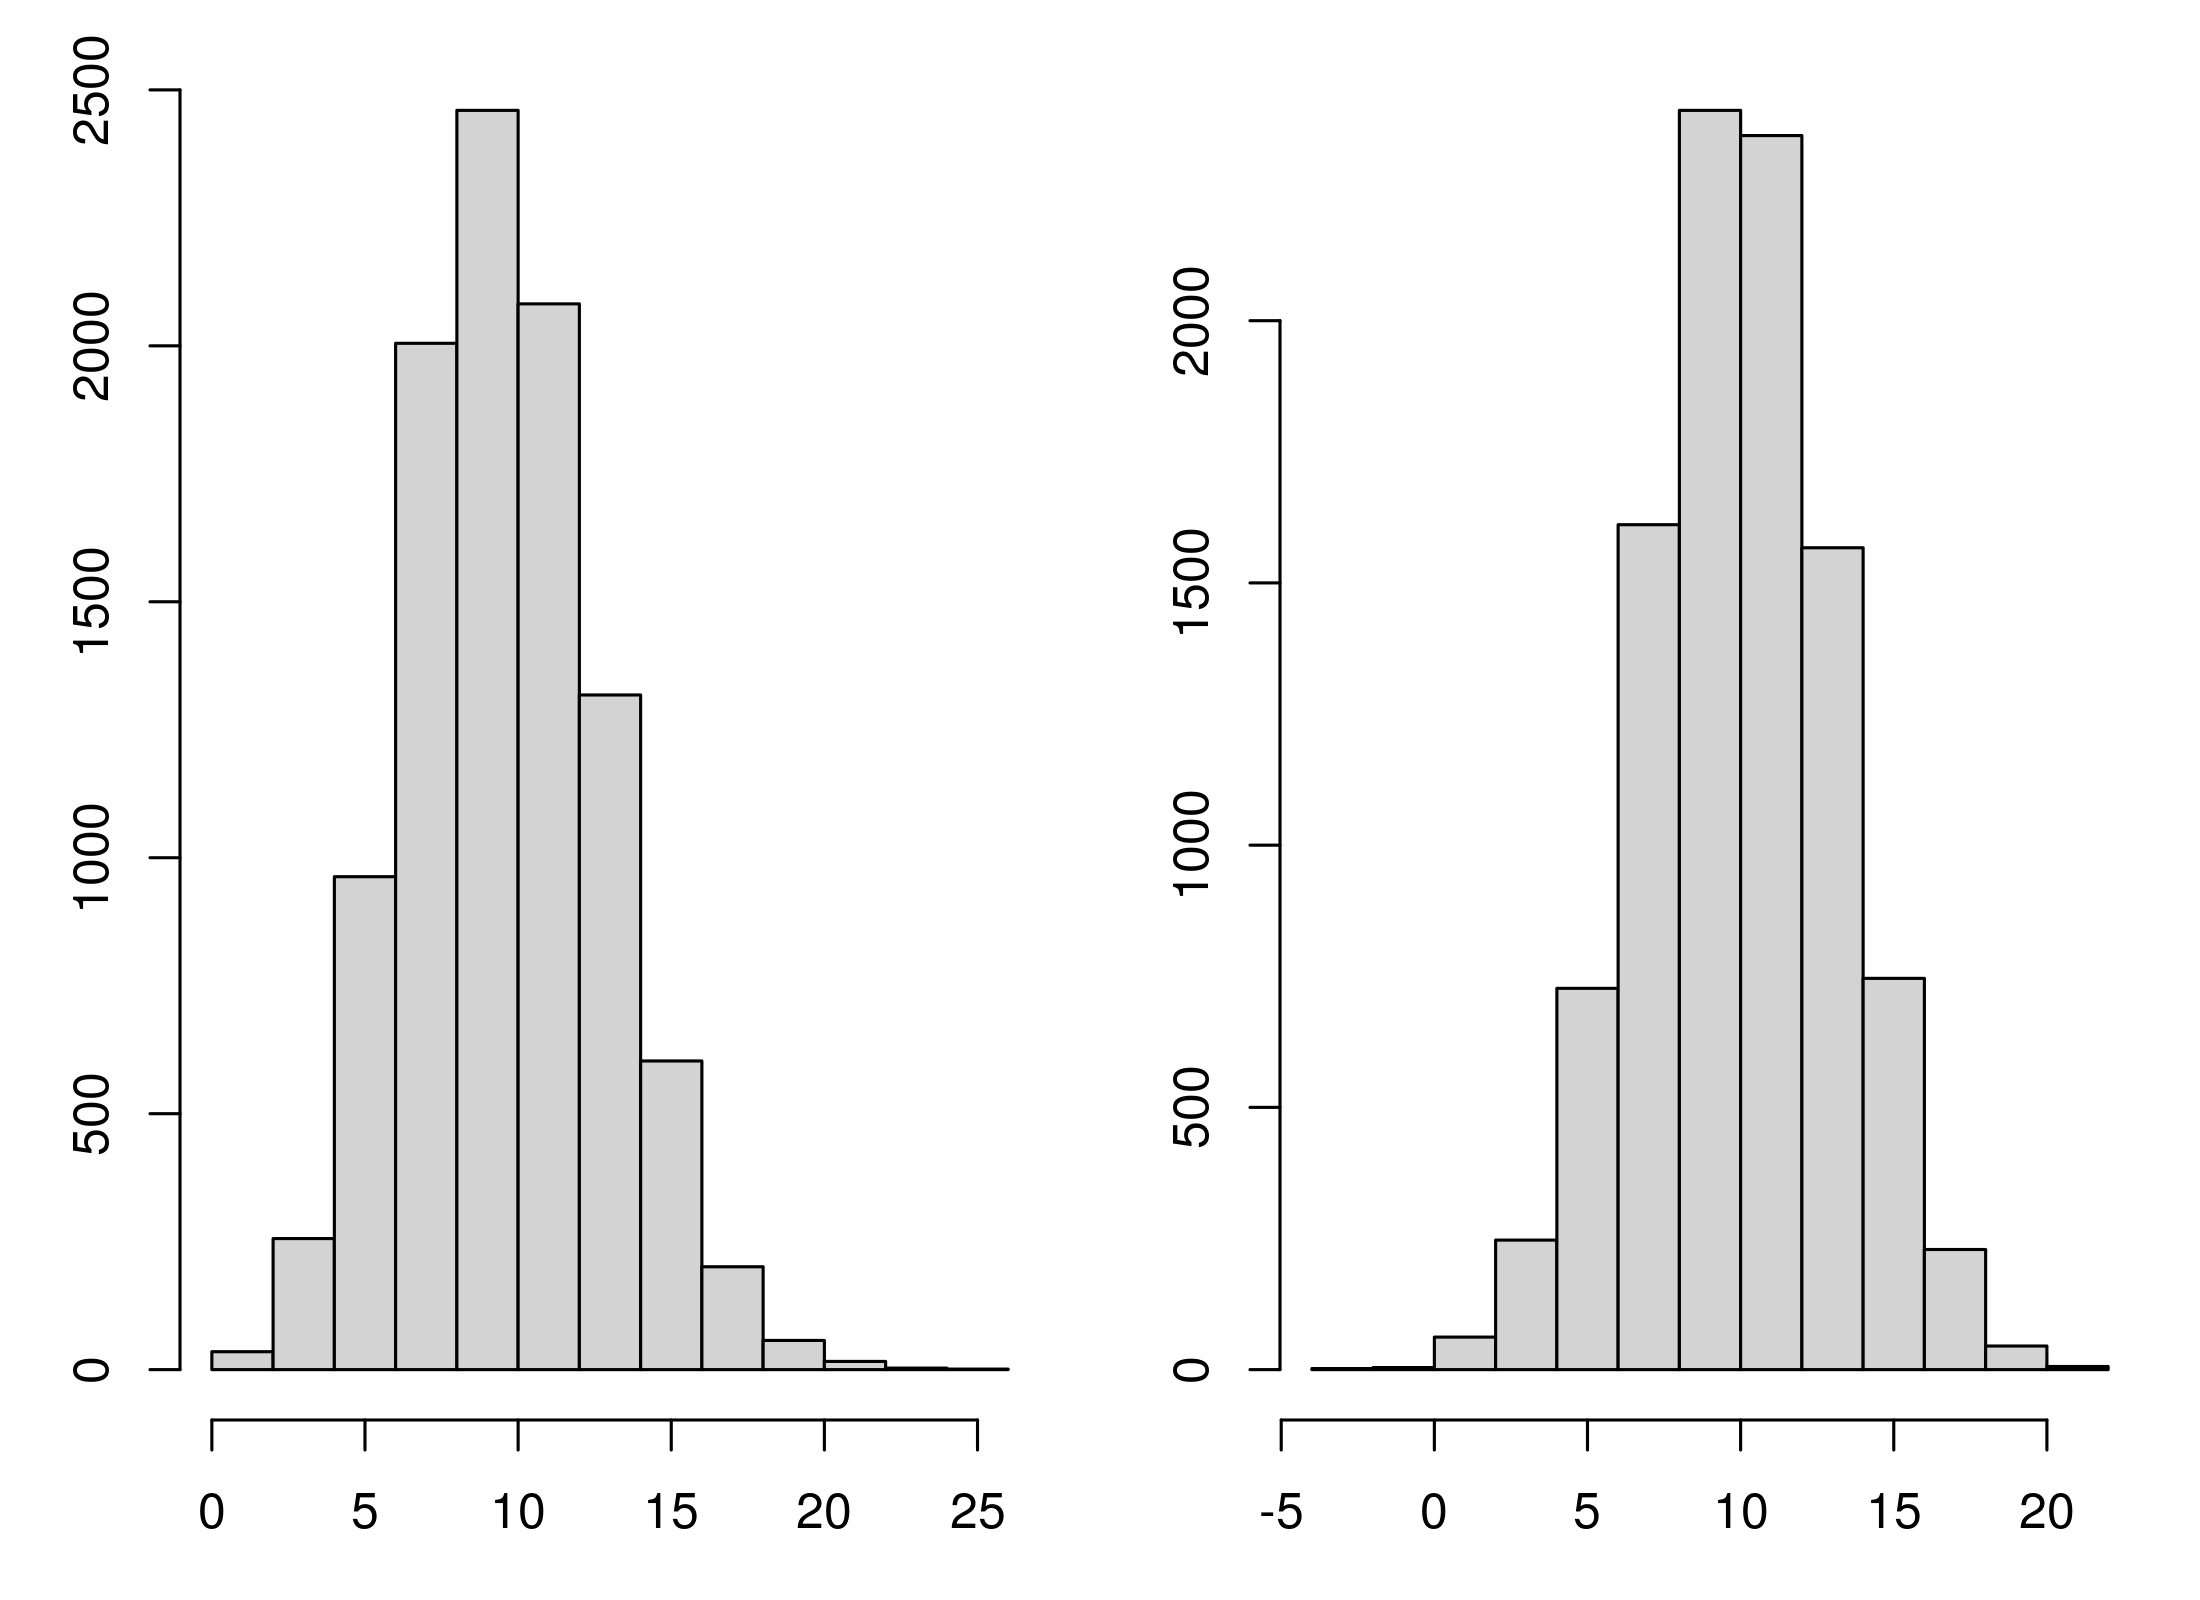
\includegraphics[scale=0.5]{poisson_normal_vl10.png}
			\caption{$\lambda=10$.}
			\label{poisson_norm10}
		\end{subfigure}
		\begin{subfigure}{\textwidth}
			\centering
			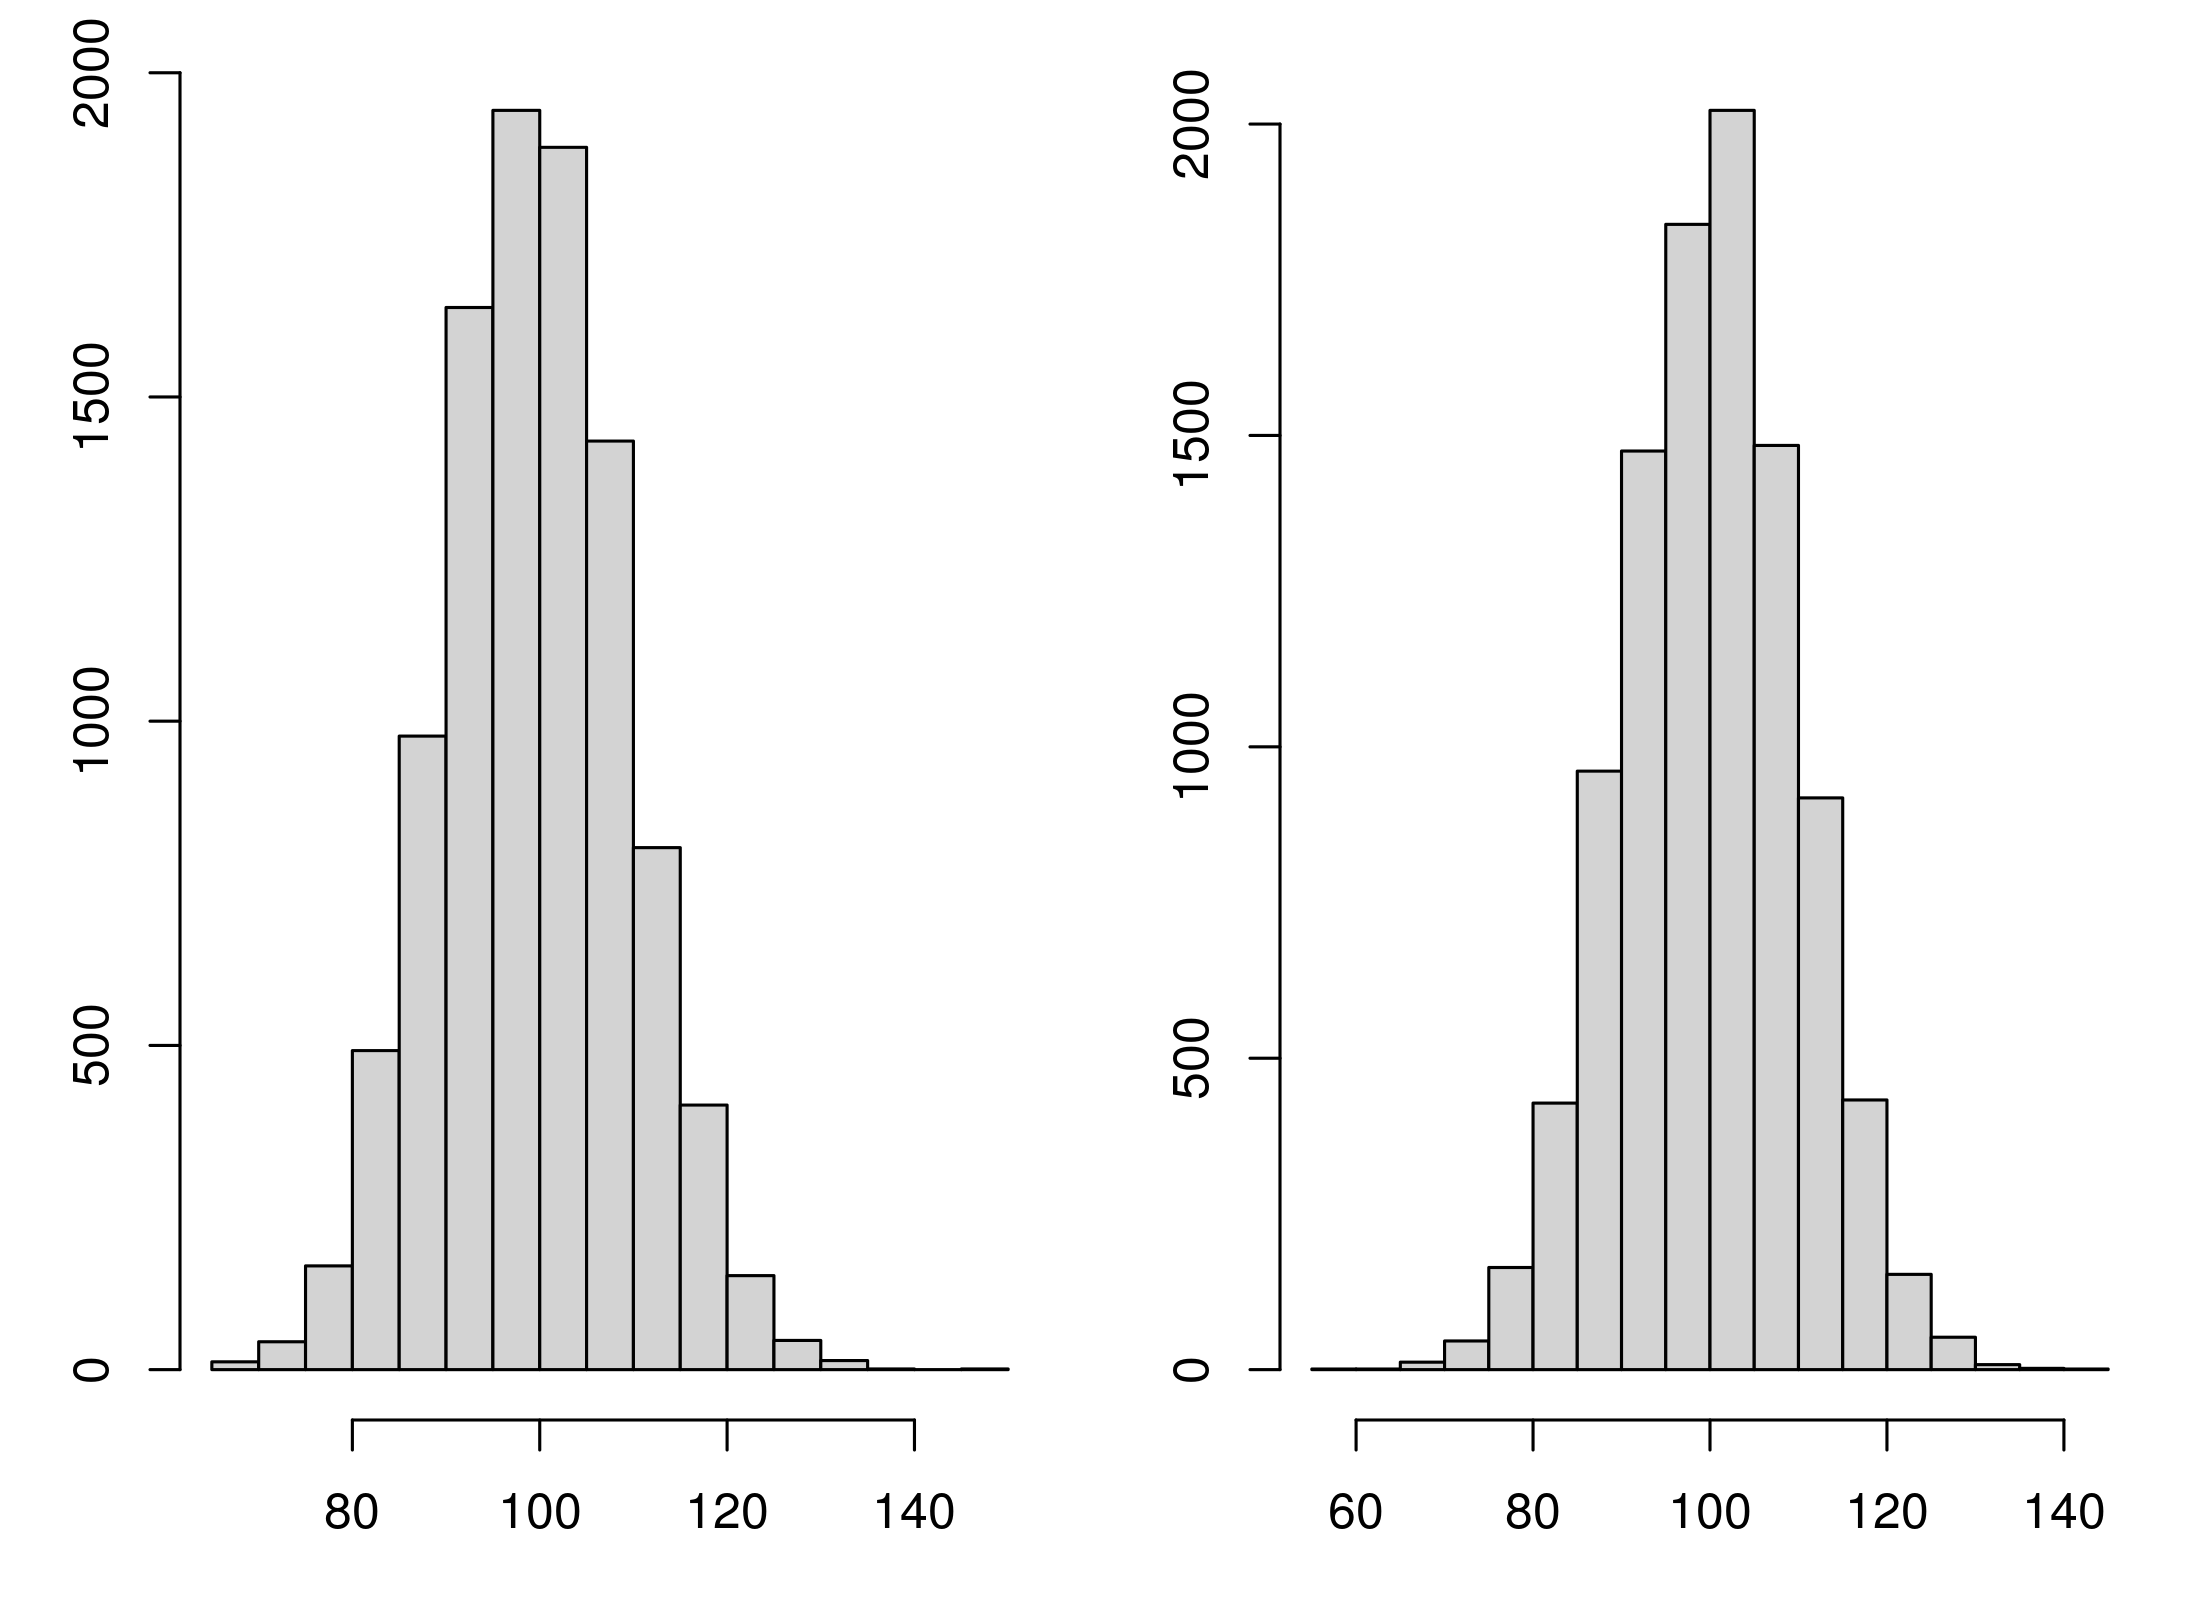
\includegraphics[scale=0.5]{poisson_normal_vl100.png}
			\caption{$\lambda = 100$.}
			\label{poisson_norm100}
		\end{subfigure}
		\caption{A la izquierda distribución de valores obtenidos con la función \texttt{rpois(r, lambda)}, a la derecha la distribución de valores con la función \texttt{rnorm(r, lambda, sqrt(lambda))}.}
		\label{poisson_norm_r}
	\end{figure}
	
	\section{Distribución de Poisson a partir de una distribución exponencial}
	
	Se continua con la idea aplicada en los casos anteriores. Se suman valores obtenidos de una distribución exponencial y se cuenta cuántos son necesarios para alcanzar una {\em meta}, que en este caso se fija en la unidad al igual que $\lambda$. El número de veces que se repite el experimento es $r=10000$.
	
	Los resultados se muestran en la figura \ref{poisson_exp}. El procedimiento está sumando valores exponencialmente distribuidos requeridos para completar un valor unitario lo que, por definición, sigue una distribución de Poisson. 
	
	\begin{figure}
		\centering
		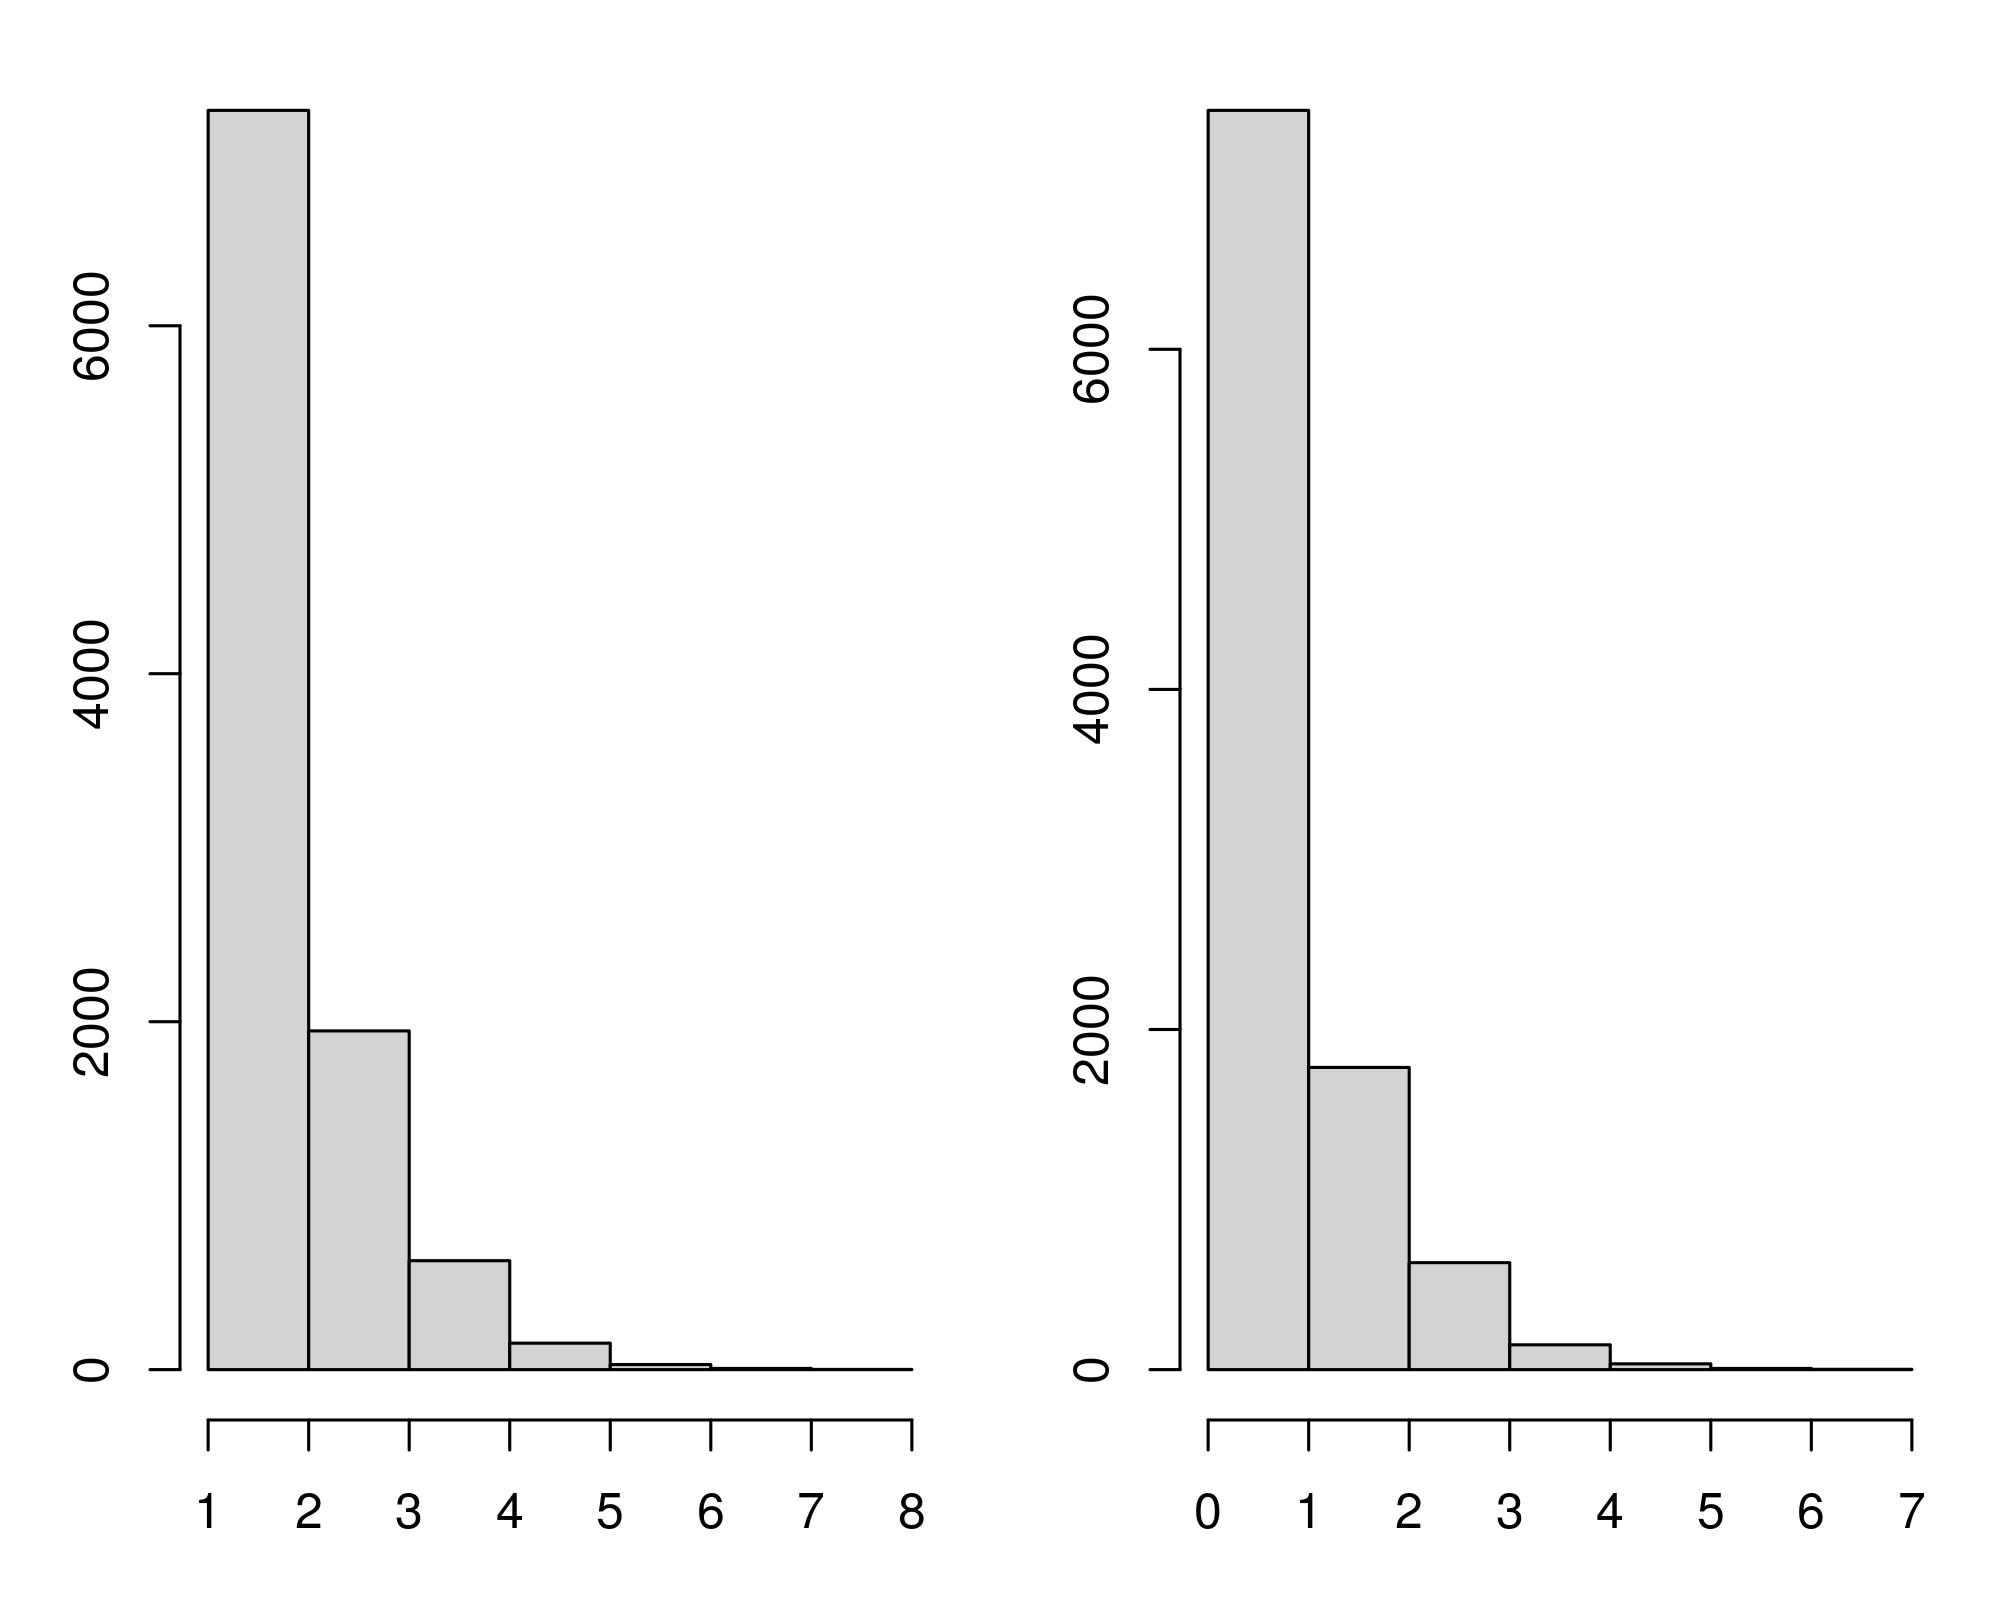
\includegraphics[scale=0.6]{poisson_exponencial.png}
		\caption{Aproximación a la distribución de Poisson a partir de la distribución exponencial. A la izquierda se encuentra la aproximación y a la derecha la distribución usando \texttt{rpois(r, 1)}}
		\label{poisson_exp}
	\end{figure}
	
	
	%\subsection*{Experimento fallido}
	
	%Se deseaba encontrar algo en el texto {\em Anne of Green Gables} que siguiera una distribución de Poisson. 
	
\bibliographystyle{plain}
\bibliography{biblio}

\end{document}

